\chapter{Hiện thực SoC và Tích hợp hệ thống}
\label{ch:soc_impl}

\textit{Chương này trình bày chi tiết quá trình hiện thực hệ thống SoC trên nền tảng FPGA. Nội dung bao gồm việc tích hợp lõi vi xử lý RISC-V, thiết kế các khối ngoại vi (Camera, DMA, UART), xây dựng hệ thống Bus kết nối và phát triển lớp phần mềm điều khiển (Firmware) để vận hành toàn bộ hệ thống.}

\section{Môi trường và Công cụ hiện thực}
% Mô tả Vivado, board FPGA sử dụng, toolchain GCC cho RISC-V
% File: 5_hien_thuc_soc/5.1_moi_truong_hien_thuc.tex

Để quá trình hiện thực hóa hệ thống SoC diễn ra đồng bộ và chính xác từ mức thiết kế phần cứng (RTL) đến lớp phần mềm điều khiển (Firmware), đề tài sử dụng một hệ thống các công cụ chuyên dụng, đảm bảo tính tương thích chặt chẽ giữa kiến trúc tập lệnh RISC-V và nền tảng FPGA.

\subsection{Môi trường thiết kế và kiểm thử phần cứng}
Quá trình thiết kế logic cho hệ thống SoC được thực hiện chủ yếu trong môi trường \textbf{Xilinx Vivado Design Suite}. Đây là nền tảng thiết kế tích hợp (IDE) cho phép quản lý các khối IP tùy biến, thực hiện các bước từ phân tích logic, tổng hợp (Synthesis) cho đến việc tối ưu hóa và hiện thực hóa (Implementation). Toàn bộ các phân hệ chức năng, bao gồm lõi xử lý PicoRV32, hệ thống Bus, Video Streaming và các bộ điều khiển ngoại vi như UART, SPI, I2C, OSPI, TIMER, GPIO đều được mô tả bằng ngôn ngữ \textbf{Verilog HDL}. Việc sử dụng ngôn ngữ mô tả phần cứng ở mức thanh ghi (RTL) giúp nhóm thiết kế kiểm soát chính xác tài nguyên logic trên FPGA và hướng tới ASIC, đảm bảo hệ thống đáp ứng được các ràng buộc khắt khe về định thời (Timing constraints) để vận hành ổn định tại tần số 200 MHz.

Trong giai đoạn xác minh thiết kế, công cụ \textbf{Vivado Simulator} đóng vai trò then chốt trong việc kiểm tra tính đúng đắn về mặt chức năng (Functional Verification). Tất cả các khối IP tự thiết kế đều phải trải qua quá trình mô phỏng thông qua hệ thống Testbench trước khi tích hợp vào hệ thống tổng thể. Quy trình này cho phép phát hiện sớm các lỗi về giao thức bắt tay trên bus AXI, logic điều phối dữ liệu của bộ gia tốc CNN và khả năng xử lý dòng dữ liệu của hệ thống Video Streaming. Đối với các lỗi phát sinh trong điều kiện thực tế trên phần cứng, lõi \textbf{Integrated Logic Analyzer (ILA)} được nhúng trực tiếp vào trong chip để giám sát các tín hiệu nội bộ theo thời gian thực, giúp gỡ lỗi các giao tiếp vật lý phức tạp như Camera/HDMI DVP, AXI,....

% File: 5_hien_thuc_soc/5.1_moi_truong_hien_thuc.tex

\subsection{Môi trường phát triển phần mềm và quy trình nhúng mã}
Phần mềm điều khiển hệ thống được phát triển dựa trên ngôn ngữ C/C++ tiêu chuẩn, cho phép tận dụng hệ sinh thái mã nguồn mở phong phú của kiến trúc RISC-V. Để chuyển đổi mã nguồn thành các tệp thực thi tương thích với phần cứng đề xuất, đề tài sử dụng bộ công cụ \textbf{RISC-V GNU Toolchain}. Trình biên dịch \texttt{riscv32-unknown-elf-gcc} được cấu hình với tham số \textbf{-march=rv32im} và \textbf{-mabi=ilp32}, tạo ra mã máy tối ưu hóa cho tập lệnh số nguyên cơ bản của lõi PicoRV32.

Điểm cốt lõi trong quy trình hiện thực hóa phần mềm là cơ chế nạp chương trình hai giai đoạn, giúp biến SoC từ một thiết kế phần cứng cố định thành một nền tảng lập trình nhúng đa năng. Trong giai đoạn tổng hợp trên Vivado, chỉ có khối bộ nhớ khởi động \textbf{BMEM} được nhúng sẵn chương trình \textbf{Bootloader} dưới dạng tệp tin Instruction Hex (.hex). Ngay khi hệ thống khởi vận, chương trình Bootloader này sẽ tự động thiết lập các giao thức cần thiết để đọc dữ liệu từ bộ nhớ Flash ngoại vi và chuyển vào bộ nhớ lệnh \textbf{IMEM}.

Cơ chế này mang lại sự thuận tiện vượt trội cho người dùng trong quá trình phát triển ứng dụng. Thay vì phải tái tổng hợp (Re-synthesis) và nạp lại toàn bộ tệp tin cấu hình FPGA (\texttt{.bit}) mỗi khi thay đổi phần mềm — một quy trình vốn tiêu tốn nhiều thời gian — người lập trình chỉ cần biên dịch chương trình C/C++ mới và cập nhật vào bộ nhớ Flash. Sau khi hoàn tất quá trình nạp dữ liệu vào IMEM, Bootloader sẽ thực hiện lệnh nhảy tới địa chỉ khởi chạy ứng dụng. Giải pháp này giúp tách biệt hoàn toàn giữa lớp hạ tầng phần cứng và lớp ứng dụng người dùng, tạo điều kiện cho việc gỡ lỗi nhanh chóng và triển khai linh hoạt các bài toán khác nhau, từ quản trị hệ thống đơn thuần đến các thuật toán xử lý dữ liệu phức tạp.

\section{Tích hợp Lõi RISC-V và Hệ thống Bus}
% Phần này mô tả backbone của hệ thống:
% - Cấu hình Core (Clock, Reset, Boot address).
% - Cấu hình AXI Interconnect/Crossbar (Phân giải địa chỉ Master/Slave).
% File: 5_hien_thuc_soc/5.2_tich_hop_loi_riscv.tex

% \section{Tích hợp Lõi RISC-V}

\subsection{Khái quát về lõi vi xử lý PicoRV32}
Trái tim của hệ thống SoC được xây dựng dựa trên lõi \textbf{PicoRV32}, một hiện thực vi xử lý mã nguồn mở tuân thủ kiến trúc tập lệnh (ISA) RISC-V. Được thiết kế với mục tiêu tối ưu hóa tài nguyên logic, PicoRV32 đặc biệt phù hợp cho các hệ thống nhúng đòi hỏi kích thước nhỏ gọn nhưng vẫn duy trì được tần số xung nhịp cao. Trong đề tài này, nhóm thiết kế lựa chọn phiên bản \textbf{picorv32\_axi} để hiện thực hóa việc kết nối. Khác với phiên bản giao tiếp bộ nhớ trực tiếp thông thường, biến thể này tích hợp sẵn giao diện bus chuẩn \textbf{AXI4} (Advanced eXtensible Interface), cho phép vi xử lý tương tác đồng bộ với hạ tầng Interconnect và các ngoại vi phức tạp trong hệ thống thông qua các giao thức bắt tay (handshake) tiêu chuẩn.

\subsection{Phân tích cấu hình và tùy chọn tập lệnh}
Để đạt được sự cân bằng giữa hiệu năng tính toán và mức tiêu thụ tài nguyên trên FPGA, lõi PicoRV32 được cấu hình thông qua một hệ thống các tham số (\textit{parameters}) chuyên biệt. Về năng lực xử lý số học, mặc dù hệ thống dựa trên nền tảng cơ bản là tập lệnh số nguyên 32-bit (\textbf{RV32I}), đề tài quyết định kích hoạt các khối tính toán phần cứng cho phép nhân và phép chia thông qua tham số \texttt{ENABLE\_MUL} và \texttt{ENABLE\_DIV}. Việc chuyển đổi sang tập lệnh \textbf{RV32IM} này đóng vai trò then chốt trong việc tăng tốc các thuật toán xử lý dữ liệu mà không cần phụ thuộc vào các thư viện phần mềm mô phỏng phép tính, vốn thường gây trễ lớn trong các ứng dụng thời gian thực. Ngược lại, tập lệnh nén (\texttt{COMPRESSED\_ISA}) được thiết lập ở mức 0 để giữ cho logic giải mã lệnh đơn giản, ưu tiên độ ổn định về định thời tại tần số 200 MHz.

Về quản lý tài nguyên nội tại, hệ thống tận dụng tối đa khả năng của lõi thông qua việc kích hoạt đầy đủ 32 thanh ghi đa năng và cơ chế truy xuất hai cổng (\texttt{ENABLE\_REGS\_DUALPORT}), giúp tối ưu hóa luồng thực thi lệnh trong ALU. Bên cạnh đó, các bộ đếm hiệu năng (\texttt{ENABLE\_COUNTERS}) cũng được tích hợp để phục vụ quá trình đo đạc thời gian thực thi của các đoạn mã điều khiển. Nhằm đảm bảo an toàn hệ thống, các cơ chế bẫy lỗi như bắt lỗi lệnh không hợp lệ (\texttt{CATCH\_ILLINSN}) và lỗi căn chỉnh bộ nhớ (\texttt{CATCH\_MISALIGN}) luôn ở trạng thái hoạt động, cho phép hệ thống tự động nhảy vào trạng thái bảo vệ (Trap) khi xảy ra sự cố phần mềm.

\subsection{Thiết lập ngữ cảnh thực thi và kết nối hệ thống}
Một khía cạnh quan trọng trong việc tích hợp lõi là quy hoạch địa chỉ khởi vận và không gian ngăn xếp để phù hợp với Memory Map toàn cục. Tham số \texttt{PROGADDR\_RESET} được thiết lập tại địa chỉ \texttt{32'h0100\_0000}, trỏ trực tiếp vào vùng nhớ \textbf{BMEM} nơi chứa chương trình Bootloader. Điều này đảm bảo ngay sau khi tín hiệu Reset được giải phóng, CPU sẽ bắt đầu quy trình nạp chương trình ứng dụng từ Flash vào IMEM như đã thiết kế. Đồng thời, địa chỉ đỉnh ngăn xếp (\texttt{STACKADDR}) được ấn định tại \texttt{32'h0001\_0000} trong vùng nhớ dữ liệu DMEM, cung cấp không gian lưu trữ an toàn cho các biến cục bộ và ngữ cảnh hàm của ngôn ngữ C.

Trong quá trình hiện thực kết nối vật lý, lõi \texttt{cpu0} được ánh xạ các tín hiệu giao diện AXI4 bao gồm các kênh địa chỉ ghi (\texttt{awaddr}), dữ liệu ghi (\texttt{wdata}), địa chỉ đọc (\texttt{araddr}) và dữ liệu đọc (\texttt{rdata}). Sự phối hợp giữa các tín hiệu \texttt{valid} và \texttt{ready} trên bus đảm bảo rằng mọi giao dịch truy xuất giữa vi xử lý và các ngoại vi như UART, I2C hay bộ gia tốc AI đều diễn ra chính xác theo đúng chu kỳ xung nhịp hệ thống. Mặc dù cơ chế ngắt (\texttt{IRQ}) được hỗ trợ về mặt logic, trong thiết kế hiện tại, các chân ngắt được giữ ở mức 0 để tập trung vào cơ chế thăm dò (\textit{Polling}) chủ động, giúp đơn giản hóa lớp trình điều khiển thiết bị trong giai đoạn phát triển ban đầu.


% File: 5_hien_thuc_soc/5.2.2_cau_hinh_chi_tiet.tex

\subsubsection{Chi tiết thiết lập tham số phần cứng (Parameters)}

Để lõi vi xử lý PicoRV32 vận hành tối ưu trong hệ thống SoC, các tham số cấu hình được thiết lập cụ thể nhằm cân bằng giữa tài nguyên logic và hiệu năng. Bảng \ref{tab:picorv32_full_params} liệt kê các tham số chính được sử dụng trong quá trình hiện thực thực thể \texttt{picorv32\_axi}.

\begin{table}[H]
    \centering % Căn giữa toàn bộ bảng trên trang giấy
    \caption{Cấu hình tham số phần cứng cho lõi PicoRV32}
    \label{tab:picorv32_full_params}
    \renewcommand{\arraystretch}{1.3}
    
    % Thiết lập độ rộng cột để không tràn lề (Tổng 14.5cm)
    \begin{tabular}{|p{4.5cm}|p{3.0cm}|p{7.0cm}|}
        \hline
        % Căn giữa tiêu đề của từng cột
        \multicolumn{1}{|c|}{\textbf{Tham số (Parameter)}} & 
        \multicolumn{1}{|c|}{\textbf{Giá trị}} & 
        \multicolumn{1}{|c|}{\textbf{Mô tả chức năng}} \\ \hline
        
        \texttt{ENABLE\_MUL} & \multicolumn{1}{|c|}{1} & Kích hoạt bộ nhân phần cứng (RV32M). \\ \hline
        \texttt{ENABLE\_DIV} & \multicolumn{1}{|c|}{1} & Kích hoạt bộ chia phần cứng (RV32M). \\ \hline
        \texttt{COMPRESSED\_ISA} & \multicolumn{1}{|c|}{0} & Không sử dụng tập lệnh nén (C). \\ \hline
        \texttt{BARREL\_SHIFTER} & \multicolumn{1}{|c|}{0} & Tối ưu diện tích, dịch bit theo chu kỳ. \\ \hline
        
        \texttt{ENABLE\_REGS\_16\_31} & \multicolumn{1}{|c|}{1} & Sử dụng đầy đủ 32 thanh ghi RV32I. \\ \hline
        \texttt{ENABLE\_REGS\_DUALPORT} & \multicolumn{1}{|c|}{1} & Hỗ trợ truy xuất đồng thời hai thanh ghi. \\ \hline
        \texttt{ENABLE\_COUNTERS} & \multicolumn{1}{|c|}{1} & Kích hoạt bộ đếm hiệu năng hệ thống. \\ \hline
        
        \texttt{CATCH\_MISALIGN} & \multicolumn{1}{|c|}{1} & Bắt lỗi truy cập bộ nhớ không căn chỉnh. \\ \hline
        \texttt{CATCH\_ILLINSN} & \multicolumn{1}{|c|}{1} & Bẫy lỗi khi gặp tập lệnh không hợp lệ. \\ \hline
        \texttt{REGS\_INIT\_ZERO} & \multicolumn{1}{|c|}{1} & Khởi tạo giá trị thanh ghi bằng 0 khi Reset. \\ \hline
        
        \texttt{PROGADDR\_RESET} & \multicolumn{1}{|c|}{\texttt{0x0100\_0000}} & Địa chỉ nạp chương trình Bootloader. \\ \hline
        \texttt{STACKADDR} & \multicolumn{1}{|c|}{\texttt{0x0001\_0000}} & Địa chỉ đỉnh ngăn xếp trong vùng DMEM. \\ \hline
    \end{tabular}
\end{table}

Việc thiết lập các tham số trên biến lõi xử lý thành kiến trúc \textbf{RV32IM}. Điều này cho phép SoC thực hiện các phép toán số học phức tạp một cách nhanh chóng, đóng vai trò quan trọng trong việc điều phối các thuật toán xử lý dữ liệu. Để đảm bảo hệ thống đạt được tần số 200 MHz, tham số \texttt{BARREL\_SHIFTER} được đặt bằng 0 nhằm giảm mức độ phức tạp của logic tổ hợp, giúp thiết kế đạt được các ràng buộc về mặt định thời trên FPGA.

\section{Thiết kế và Tích hợp các khối Ngoại vi}
% Đây là phần trọng tâm công việc của bạn (System Design):
% - Khối DMA Controller (Để chuyển ảnh).
% - Khối DVP Interface (Giao tiếp Camera).
% - Các khối cơ bản: UART, SPI, GPIO, Timer.
% File: 5_hien_thuc_soc/5.4_ngoai_vi_uart.tex

% \section{Thiết kế và Tích hợp các khối Ngoại vi}


\subsection{UART}

Khối UART được thiết kế để đảm nhiệm vai trò kênh giao tiếp gỡ lỗi (Console/Debug) và truyền nhận dữ liệu tốc độ thấp. Toàn bộ khối IP được xây dựng theo kiến trúc phân lớp, từ các tầng vật lý xử lý tín hiệu nối tiếp đến tầng giao diện thanh ghi tương thích chuẩn AXI.

\subsubsection{Kiến trúc hệ thống và bộ tạo tốc độ Baud}
Cấu trúc tổng quát của ngoại vi UART dựa trên module \textbf{uart\_unit}, tích hợp các thành phần cốt lõi bao gồm bộ tạo tốc độ Baud, khối transmitter/receiver và các bộ đệm FIFO hàng đợi.




\begin{figure}[H]
    \centering
    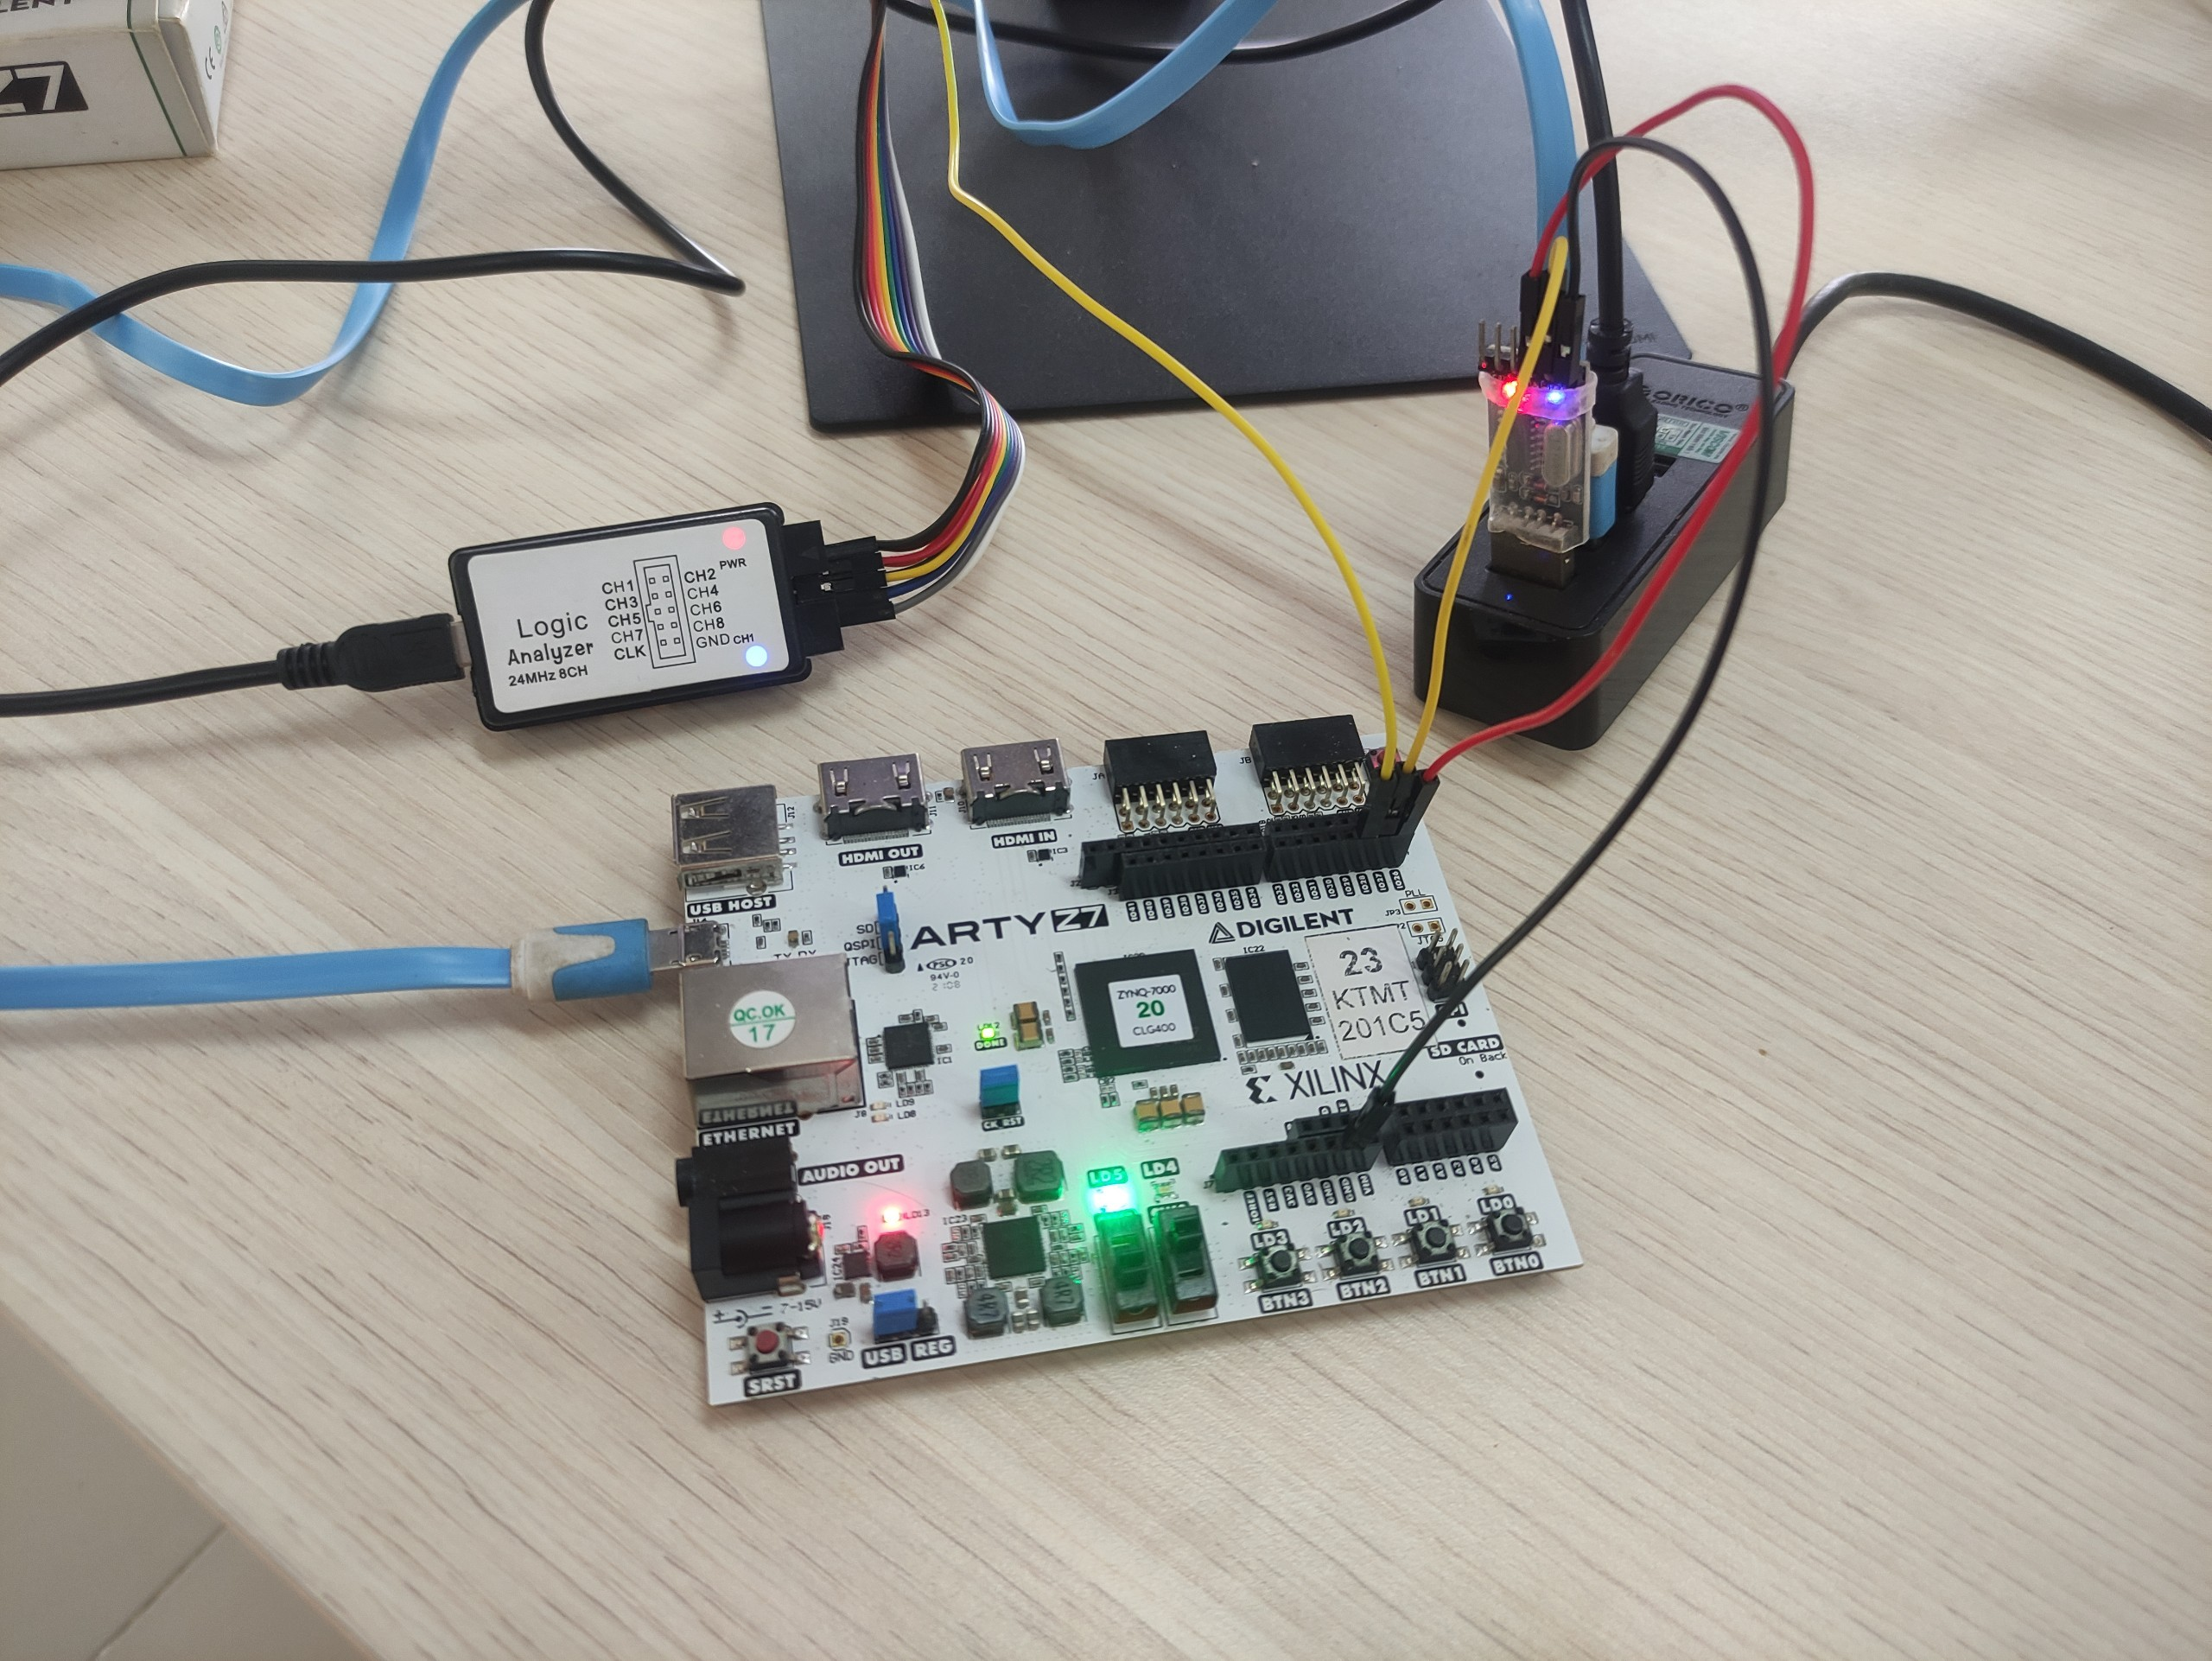
\includegraphics[width=1\textwidth]{5_hien_thuc_soc/image/uart.png}
    \caption{Sơ đồ khối kiến trúc module UART Unit}
    \label{fig:uart_architecture}
\end{figure}

% File: 5_hien_thuc_soc/5.4_ngoai_vi_uart.tex

Nền tảng vận hành của khối UART là module \textbf{buad\_gen}, đóng vai trò như một bộ chia tần số linh hoạt. Với xung nhịp hệ thống cao (200 MHz), bộ tạo tốc độ Baud sử dụng một thanh ghi đếm và một thanh ghi giá trị chia (\texttt{dvsr}) để tạo ra các xung \texttt{tick} định thời. Các xung này được thiết lập tại tần số gấp 16 lần tốc độ Baud mục tiêu (Oversampling), cho phép khối nhận (\textit{Receiver}) thực hiện lấy mẫu dữ liệu chính xác tại trung tâm của mỗi bit truyền. Cơ chế này giúp tăng cường khả năng chống nhiễu và bù đắp sai số xung nhịp giữa SoC và các thiết bị ngoại vi giao tiếp.

Giá trị nạp vào thanh ghi cấu hình \texttt{dvsr} được xác định dựa trên mối tương quan giữa tần số hệ thống và tốc độ truyền thông mong muốn thông qua công thức sau:

\begin{equation}
    v = \frac{f_{clk}}{16 \times B} - 1
\end{equation}

Trong đó các tham số được định nghĩa cụ thể:
\begin{itemize}
    \item \textbf{$v$}: Giá trị số nguyên được nạp vào thanh ghi \texttt{dvsr} của bộ tạo Baud.
    \item \textbf{$f_{clk}$}: Tần số xung nhịp hệ thống đầu vào (trong thiết kế này là 200 MHz).
    \item \textbf{$B$}: Tốc độ Baud mong muốn (ví dụ: 9600, 115200 bits/second).
    \item \textbf{16}: Hệ số lấy mẫu dư (Oversampling factor) cố định, đảm bảo bộ nhận UART lấy mẫu mỗi bit 16 lần để tối ưu hóa độ chính xác.
\end{itemize}

Ví dụ, với tần số hệ thống $f_{clk} = 100$ MHz và tốc độ Baud yêu cầu $B = 9600$, giá trị $v$ tính toán được xấp xỉ 650. Đối với cấu hình thực tế của đề tài tại tần số 200 MHz và tốc độ 115200 bps, giá trị này sẽ được phần mềm tính toán và nạp vào thanh ghi điều khiển tương ứng tại thời điểm khởi tạo hệ thống.

% \begin{figure}[H]
%     \centering
%     \includegraphics[width=0.8\textwidth]{5_hien_thuc_soc/image/uart1.png}
%     \caption{Sơ đồ khối và logic tính toán của bộ tạo tốc độ Baud}
%     \label{fig:uart_baud_gen}
% \end{figure}

\subsubsection{Hiện thực máy trạng thái cho bộ nhận (RX) và bộ truyền (TX)}
Logic truyền nhận vật lý được điều khiển bởi các máy trạng thái hữu hạn (FSM) trong module \textbf{uart\_rx} và \textbf{uart\_tx}. 

Đối với bộ nhận, FSM hoạt động qua 4 trạng thái chính: \textit{IDLE, START, DATA} và \textit{STOP}. Khi phát hiện Start-bit, hệ thống sẽ đếm 7 xung \texttt{tick} để nhảy vào giữa bit và sau đó cứ mỗi 16 xung \texttt{tick} sẽ thực hiện lấy mẫu một bit dữ liệu. Quy trình này đảm bảo dữ liệu được thu thập tại thời điểm tín hiệu ổn định nhất.



\begin{figure}[H]
    \centering
    \includegraphics[width=1.2\textwidth]{5_hien_thuc_soc/image/uart2.png}
    \caption{Sơ đồ máy trạng thái (FSM) của bộ nhận UART RX}
    \label{fig:uart_fsm_rx}
\end{figure}

Tương tự, bộ truyền \textbf{uart\_tx} thực hiện quá trình chuyển đổi từ dữ liệu song song 8-bit sang khung truyền nối tiếp. Dữ liệu được đẩy ra chân \texttt{tx} kèm theo các bit khung (Start/Stop) theo đúng định thời được cấu hình, đảm bảo tính đồng bộ hoàn toàn với thiết bị đầu cuối.

\subsubsection{Cơ chế đệm dữ liệu và quản lý dòng thông tin}
Nhằm tối ưu hóa hiệu suất cho CPU, hệ thống tích hợp các khối \textbf{fifo\_unit} cho cả hai chiều truyền và nhận. Với độ sâu được thiết lập qua tham số \texttt{FIFO\_W}, các bộ đệm này cho phép CPU có thể nạp một chuỗi dữ liệu dài vào hàng đợi và tiếp tục thực thi các thuật toán AI mà không cần chờ đợi từng byte được truyền xong. 

% \begin{figure}[H]
%     \centering
%     % \includegraphics[width=0.7\textwidth]{figures/uart_fifo_flow.png}
%     \caption{Luồng dữ liệu giữa vi xử lý và UART thông qua hàng đợi FIFO}
%     \label{fig:uart_fifo_flow}
% \end{figure}

Sự hiện diện của FIFO giúp triệt tiêu hiện tượng mất dữ liệu (Data Overflow) khi vi xử lý đang bận xử lý các tác vụ ưu tiên cao, đồng thời tăng băng thông tổng thể cho hệ thống giao tiếp.

\subsubsection{Tích hợp giao diện AXI4-Lite}
Việc nhúng khối UART vào hệ thống SoC được thực hiện thông qua module \textbf{uart\_axi\_lite}. Module áp dụng \textbf{axi\_lite\_slave\_interface} để ánh xạ các tài nguyên của UART thành các thanh ghi trong không gian địa chỉ của CPU.

\begin{figure}[H]
    \centering
    \includegraphics[width=0.8\textwidth]{5_hien_thuc_soc/image/uart3.png}
    \caption{Các thanh ghi kết nối giữa Bus AXI4-Lite và ngoại vi UART}
    \label{fig:uart_axi_interface}
\end{figure}

Thông qua việc truy cập vào các địa chỉ Base Address đã quy hoạch trong Memory Map, phần mềm điều khiển có thể:
\begin{itemize}
    \item Đọc dữ liệu từ hàng đợi nhận hoặc ghi dữ liệu cần gửi vào hàng đợi truyền.
    \item Kiểm tra các trạng thái hệ thống như \texttt{tx\_full} (đầy bộ đệm truyền) hoặc \texttt{rx\_empty} (hết dữ liệu nhận) để điều phối luồng chương trình.
    \item Cấu hình lại tốc độ Baud linh hoạt ngay trong quá trình vận hành bằng cách ghi giá trị mới vào thanh ghi \texttt{dvsr}.
\end{itemize}

Kiến trúc này đảm bảo tính tách biệt hoàn toàn giữa logic bus và logic truyền nhận, giúp khối ngoại vi hoạt động ổn định và dễ dàng tái sử dụng trong các thiết kế SoC khác nhau.



% File: 5_hien_thuc_soc/5.4.2_ngoai_vi_spi.tex

\subsection{SPI}

Bên cạnh UART, giao thức giao tiếp ngoại vi nối tiếp (SPI - Serial Peripheral Interface) đóng vai trò quan trọng trong việc kết nối SoC với các cảm biến tốc độ cao hoặc các bộ nhớ Flash phụ trợ. Khối IP SPI được thiết kế theo cấu trúc Master, cho phép lõi PicoRV32 chủ động điều phối luồng dữ liệu thông qua cơ chế truyền nhận đồng bộ.

\subsubsection{Cấu trúc logic và bộ tạo xung nhịp SPI}





Khác với UART sử dụng cơ chế lấy mẫu dư, SPI là một giao thức đồng bộ nên yếu tố then chốt nằm ở việc tạo ra xung nhịp \texttt{sclk} ổn định. Module tích hợp một bộ chia tần số linh hoạt, cho phép phần mềm cấu hình tốc độ truyền thông dựa trên tần số hệ thống 200 MHz. Điểm đặc biệt trong hiện thực này là khả năng tùy biến các chế độ hoạt động (\textit{SPI Modes}) thông qua việc điều chỉnh cực tính (\texttt{CPOL}) và pha của xung nhịp (\texttt{CPHA}), đảm bảo tính tương thích với đa dạng các chủng loại linh kiện ngoại vi trên thị trường.

\begin{figure}[H]
    \centering
    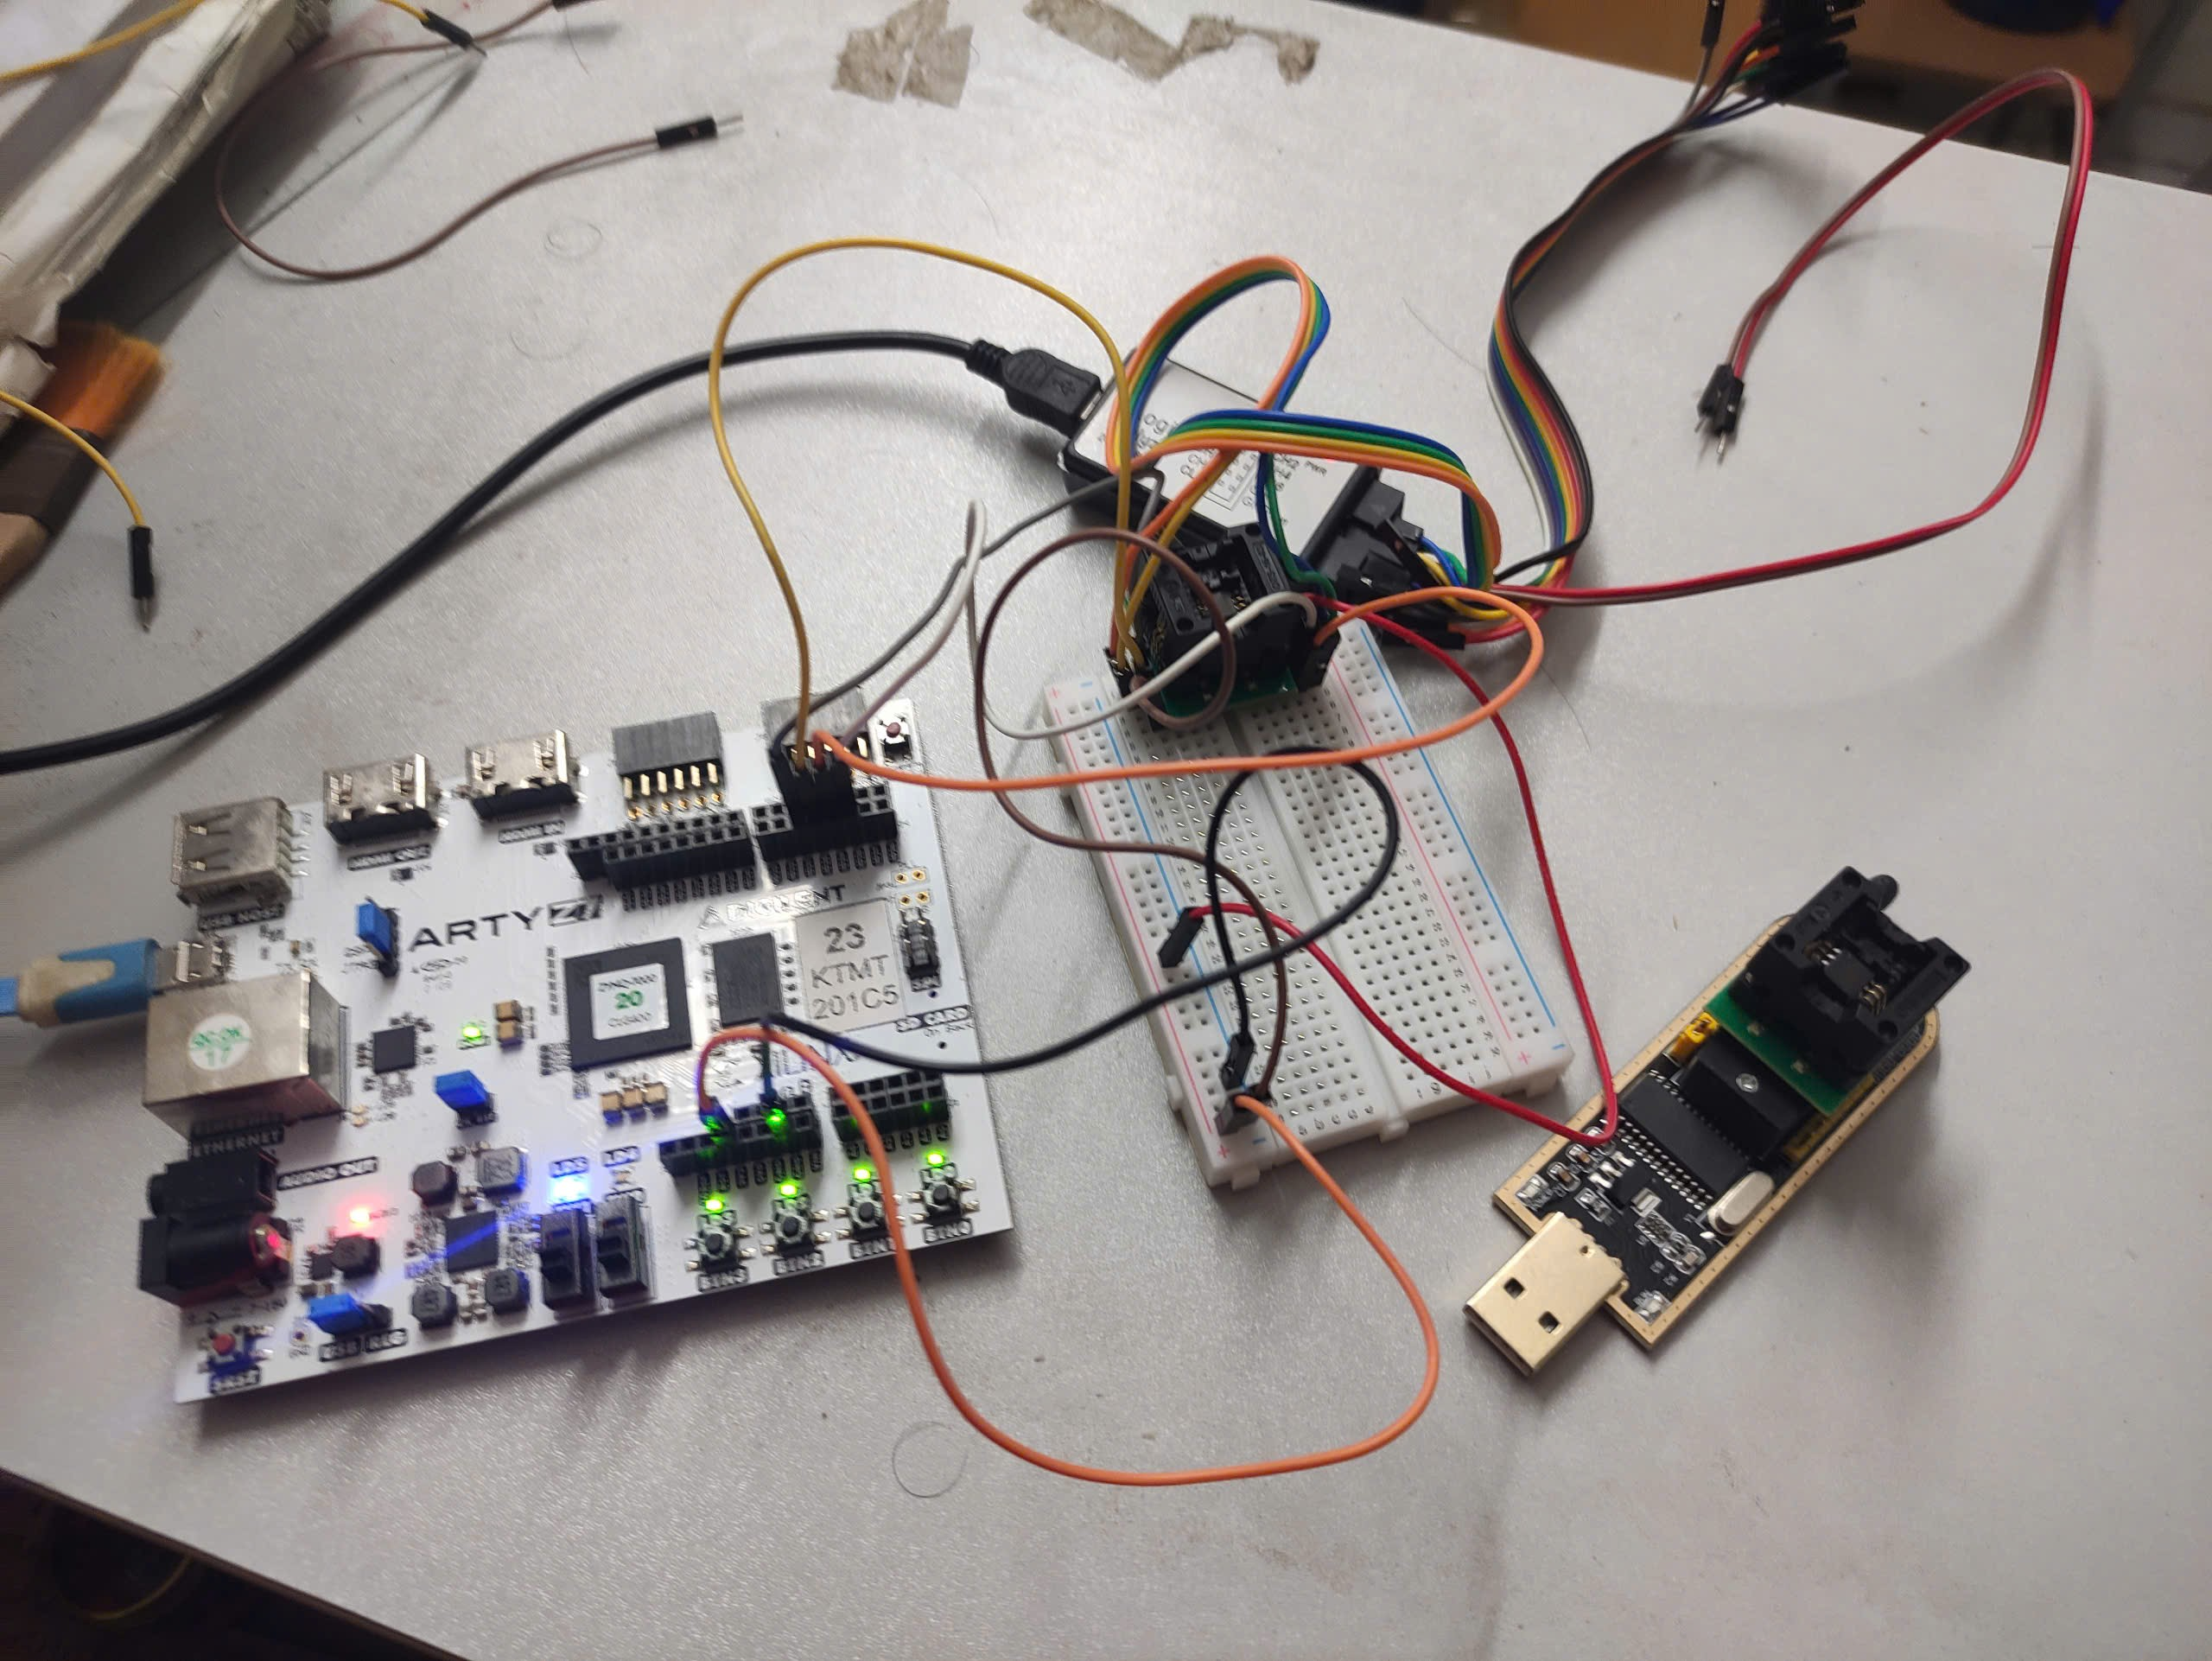
\includegraphics[width=1\textwidth]{5_hien_thuc_soc/image/spi.png}
    \caption{SPI Mode}
    \label{fig:spi_architecture}
\end{figure}


% \begin{figure}[H]
%     \centering
%     \includegraphics[width=0.8\textwidth]{5_hien_thuc_soc/image/spi1.png}
%     \caption{Sơ đồ khối ý tưởng dich bit trong SPI}
%     \label{fig:spi_architecture}
% \end{figure}
\subsubsection{Cơ chế điều khiển và Máy trạng thái FSMD}

Hệ thống SPI Master được hiện thực hóa dựa trên kiến trúc \textbf{FSMD} (Finite State Machine with Datapath), nơi bộ điều khiển máy trạng thái (FSM) đóng vai trò chỉ đạo và khối dữ liệu (Datapath) thực hiện các phép toán logic như dịch bit và đếm số bit đã truyền. Quy trình này được mô phỏng chi tiết dựa trên sơ đồ máy trạng thái và giản đồ định thời của giao thức SPI.

% \begin{figure}[H]
%     \centering
%         \caption{Sơ đồ chuyển trạng thái của khối điều khiển SPI Master}
%     \label{fig:spi_fsm}
% \end{figure}

Hoạt động của FSM bao gồm các trạng thái chính sau:
\begin{itemize}
    \item[] \textbf{Trạng thái IDLE:} Đây là trạng thái mặc định của hệ thống. Tín hiệu chọn chip \texttt{ss} được giữ ở mức cao ($Logic\ 1$) để ngắt kết nối với các Slave ngoại vi. FSM liên tục giám sát tín hiệu khởi tạo từ Bus AXI; ngay khi có lệnh truyền, hệ thống sẽ nạp dữ liệu vào thanh ghi dịch và chuyển sang trạng thái kế tiếp.
    \item[] \textbf{Trạng thái TRANSFER:} Tại đây, tín hiệu \texttt{ss} được kéo xuống thấp ($Logic\ 0$) để bắt đầu phiên làm việc. Khối Datapath bắt đầu vận hành đồng bộ với xung nhịp \texttt{sclk}.
    \begin{itemize}
        \item[] \textbf{Dịch bit dữ liệu (Shift-out):} Tại mỗi cạnh tích cực (hoặc cạnh dẫn tùy theo cấu hình CPOL/CPHA), bit có trọng số cao nhất (MSB) của thanh ghi dịch được đẩy ra chân \texttt{mosi}.
        \item[] \textbf{Lấy mẫu dữ liệu (Sample-in):} Đồng thời, tín hiệu từ chân \texttt{miso} được lấy mẫu và đưa vào vị trí bit thấp nhất (LSB) của thanh ghi dịch.
        \item[] \textbf{Bộ đếm bit:} Một bộ đếm nội bộ (\textit{Bit Counter}) theo dõi số lượng xung nhịp. Sau khi hoàn tất đủ 8 chu kỳ (tương đương 1 byte dữ liệu), FSM sẽ quyết định kết thúc hoặc tiếp tục truyền byte tiếp theo.
    \end{itemize}
    \item[] \textbf{Trạng thái DONE/READY:} Sau khi trao đổi đủ dữ liệu, tín hiệu \texttt{ss} được đưa trở lại mức cao. Đồng thời, tín hiệu \texttt{ready} sẽ được kích hoạt ở mức logic 1 trong một chu kỳ xung nhịp hệ thống để báo hiệu cho vi xử lý PicoRV32 rằng dữ liệu trong thanh ghi đã sẵn sàng để đọc hoặc byte tiếp theo có thể được nạp vào.
\end{itemize}

\begin{figure}[H]
    \centering
    \includegraphics[width=1\textwidth]{5_hien_thuc_soc/image/spi2.png}
    \caption{Thời gian thực hiện thao tác dịch dữ liệu trong SPI}
    \label{fig:spi_architecture}
\end{figure}

\begin{figure}[H]
    \centering
    \includegraphics[width=0.85\textwidth]{5_hien_thuc_soc/image/spi3.png}
    \caption{SPI controller ASMD chart}
    \label{fig:spi_architecture}
\end{figure}

Sự phối hợp chặt chẽ giữa bộ đếm và thanh ghi dịch trong tầng Datapath giúp triệt tiêu các sai số về định thời. Việc sử dụng thanh ghi đệm tại chân \texttt{miso} trước khi nạp vào FSM đảm bảo rằng dữ liệu nhận được luôn ổn định, tránh các hiện tượng nhiễu tức thời tại cạnh xung nhịp, từ đó duy trì tính toàn vẹn của dữ liệu trong suốt quá trình giao tiếp tốc độ cao với các ngoại vi.




% \begin{figure}[H]
%     \centering
%     \includegraphics[width=1\textwidth]{5_hien_thuc_soc/image/spi2.png}
%     \caption{Thời gian thực hiện thao tác dịch dữ liệu trong SPI}
%     \label{fig:spi_architecture}
% \end{figure}

% \begin{figure}[H]
%     \centering
%     \includegraphics[width=0.8\textwidth]{5_hien_thuc_soc/image/spi3.png}
%     \caption{SPI controller ASMD chart}
%     \label{fig:spi_architecture}
% \end{figure}

\subsubsection{Tích hợp hệ thống qua giao diện AXI4-Lite}
Khối SPI được nhúng vào không gian địa chỉ SoC thông qua module \textbf{Spi\_axi\_lite\_core}. Tương tự như khối UART, việc giao tiếp được thực hiện theo cơ chế nạp/lưu dữ liệu trực tiếp vào các thanh ghi chức năng (Memory-mapped I/O).

Giao diện \textbf{axi\_lite\_interface} đóng vai trò là tầng trung gian xử lý các giao thức bắt tay của bus. CPU quản lý ngoại vi SPI thông qua tập hợp các thanh ghi 32-bit sau:
\begin{itemize}
    \item[] \textbf{Thanh ghi dữ liệu (Data Register):} Chứa dữ liệu cần truyền đi hoặc dữ liệu vừa nhận về từ thiết bị tớ.
    \item[] \textbf{Thanh ghi điều khiển (Control Register):} Cho phép cấu hình tốc độ xung nhịp \texttt{sclk}, chọn thiết bị tớ (Slave Select) và thiết lập các tham số truyền thông.
    \item[] \textbf{Thanh ghi trạng thái (Status Register):} Cung cấp các cờ báo hiệu như \texttt{busy} (đang bận truyền) hoặc \texttt{done} (hoàn tất giao dịch), hỗ trợ phần mềm thực hiện cơ chế kiểm tra trạng thái chủ động (\textit{Polling}).
\end{itemize}

\begin{figure}[H]
    \centering
    \includegraphics[width=0.9\textwidth]{5_hien_thuc_soc/image/spi4.png}
    \caption{Các thanh ghi kết nối giữa Bus AXI4-Lite và ngoại vi SPI}
    \label{fig:spi_architecture}
\end{figure}

Việc sử dụng các thanh ghi đệm \textit{D-Flip-Flop} tại tầng vật lý giúp cô lập hoàn toàn logic bus hệ thống với các tín hiệu I/O bên ngoài. Thiết kế này giúp triệt tiêu các vấn đề về nhiễu tín hiệu và đảm bảo rằng hệ thống Bus AXI vẫn duy trì được hiệu suất cao tại tần số 200 MHz trong khi khối SPI có thể hoạt động tại các dải tần số thấp hơn tùy theo yêu cầu của linh kiện ngoại vi.


% File: 5_hien_thuc_soc/5.4.3_ngoai_vi_i2c.tex

\subsection{I2C}

Trong hệ thống SoC đề xuất, giao thức I2C (Inter-Integrated Circuit) đóng vai trò là kênh điều khiển thiết yếu để cấu hình các tham số vận hành cho cảm biến hình ảnh OV5640 và chip phát HDMI (ADV7513). Khối IP I2C Master được hiện thực hóa với khả năng điều khiển bus hai dây (\texttt{scl} và \texttt{sda}), hỗ trợ đa thiết bị tớ thông qua cơ chế địa chỉ hóa và bắt tay chặt chẽ.

\subsubsection{Kiến trúc bộ điều khiển I2C Master}
Thành phần hạt nhân của phân hệ là module \textbf{i2c\_master}, được thiết kế theo mô hình FSMD để quản lý các điều kiện phức tạp trên đường truyền. Khác với các giao thức nối tiếp khác, I2C sử dụng cấu trúc cực Open-drain, đòi hỏi bộ điều khiển phải quản lý linh hoạt trạng thái trở kháng cao (\textit{High-Impedance}) để cho phép các thiết bị tớ phản hồi tín hiệu Ack/Nack.




% \begin{figure}[H]
%     \centering
%     % \includegraphics[width=0.8\textwidth]{figures/i2c_architecture.png}
%     \caption{Sơ đồ khối kiến trúc bộ điều khiển I2C Master}
%     \label{fig:i2c_architecture}
% \end{figure}

Để tạo ra xung nhịp \texttt{scl} từ nền tảng 200 MHz, module tích hợp một bộ chia tần số dựa trên thanh ghi \texttt{dvsr}. Tuy nhiên, do đặc thù của I2C yêu cầu duy trì các khoảng thời gian thiết lập (\textit{Setup time}) và giữ (\textit{Hold time}) khắt khe cho điều kiện Start và Stop, bộ tạo xung được chia thành 4 giai đoạn (\textit{Quarters}) trong mỗi chu kỳ. Việc lấy mẫu tín hiệu \texttt{sda} luôn được thực hiện tại trung tâm của mức cao xung \texttt{scl} để đảm bảo tính ổn định tối đa của dữ liệu.

\begin{figure}[H]
    \centering
    \includegraphics[width=0.9\textwidth]{5_hien_thuc_soc/image/i2c.png}
    \caption{Chia các giai đoạn điều kiện trong chu kỳ xung nhịp I2C}
    \label{fig:spi_architecture}
\end{figure}

\begin{figure}[H]
    \centering
    \includegraphics[width=0.9\textwidth]{5_hien_thuc_soc/image/i2c1.png}
    \caption{Chia các giai đoạn dữ liệu trong chu kỳ xung nhịp I2C}
    \label{fig:spi_architecture}
\end{figure}

% File: 5_hien_thuc_soc/5.4.3.2_fsm_i2c.tex

\subsubsection{Hiện thực Máy trạng thái điều khiển (Control FSM)}

Máy trạng thái hữu hạn (FSM) là thành phần cốt lõi điều phối toàn bộ trình tự logic của khối I2C Master. FSM tiếp nhận tín hiệu đầu vào \texttt{cmd} để xác định loại tác vụ cần thực hiện, bao gồm: \texttt{RD\_CMD} (đọc dữ liệu), \texttt{WR\_CMD} (ghi dữ liệu), \texttt{START\_CMD} (tạo điều kiện bắt đầu), \texttt{RESTART\_CMD} (khởi động lại giao dịch) và \texttt{STOP\_CMD} (tạo điều kiện kết thúc). Các trạng thái trong FSM được thiết kế để khớp nối chính xác với các pha thời gian của giao thức I2C, đảm bảo tính ổn định cho hai đường tín hiệu \texttt{scl} và \texttt{sda}.

\begin{figure}[H]
    \centering
    \includegraphics[width=0.95\textwidth]{5_hien_thuc_soc/image/i2c2.png}
    \caption{Sơ đồ các trạng thái của bộ điều khiển I2C Master}
    \label{fig:i2c_fsm_logic}
\end{figure}

Quy trình vận hành của FSM được hiện thực hóa qua các giai đoạn cụ thể như sau:

\begin{itemize}
    \item[] \textbf{Khởi tạo giao dịch (Start Phase):} Khi nhận lệnh \texttt{START\_CMD}, FSM sẽ chuyển lần lượt qua các trạng thái \texttt{start1} và \texttt{start2}. Tại đây, bộ điều khiển sẽ tạo ra điều kiện Start bằng cách điều phối mức logic trên các chân I/O để thông báo phiên giao dịch mới cho các thiết bị trên bus.
    
    \item[] \textbf{Xử lý dữ liệu và bit xác nhận (Data Phase):} Sau khi thiết lập điều kiện Start, các lệnh \texttt{WR\_CMD} hoặc \texttt{RD\_CMD} sẽ được thực thi. Cả hai tác vụ này đều đi qua chu trình gồm 4 trạng thái: \texttt{data1}, \texttt{data2}, \texttt{data3} và \texttt{data4}.
    \begin{itemize}
        \item[] Chu trình này được lặp lại 9 lần cho mỗi byte dữ liệu (bao gồm 8 bit dữ liệu chính và 1 bit xác nhận ACK/NACK).
        \item[] Một bộ đếm nội bộ (\texttt{bit\_reg}) được sử dụng để theo dõi số lần lặp và đảm bảo trình tự dịch bit diễn ra chính xác.
        \item[] Sau khi xử lý đủ 9 bit, FSM chuyển sang trạng thái \texttt{data\_end} để kéo thấp các đường \texttt{scl} và \texttt{sda} trong một khoảng thời gian tương ứng với 1/4 chu kỳ xung nhịp trước khi chuyển về trạng thái giữ.
    \end{itemize}

    \item[] \textbf{Duy trì trạng thái (Hold State) và Phản hồi Ready:} Sau khi hoàn tất một lệnh đơn lẻ, FSM sẽ duy trì ở trạng thái \texttt{hold} để chờ đợi chỉ thị tiếp theo từ vi xử lý. Ở trạng thái này, cả \texttt{scl} và \texttt{sda} đều được giữ ở mức thấp. Tín hiệu trạng thái \texttt{ready} sẽ được kích hoạt tại các trạng thái \texttt{idle} hoặc \texttt{hold} để báo hiệu cho lõi PicoRV32 rằng bộ điều khiển đã sẵn sàng nhận lệnh mới.

    \item[] \textbf{Kết thúc hoặc Khởi động lại (Stop/Restart Phase):} Giao dịch được kết thúc bằng lệnh \texttt{STOP\_CMD}, buộc FSM đi qua các trạng thái \texttt{stop1} và \texttt{stop2} để tạo điều kiện Stop. Nếu nhận lệnh \texttt{RESTART\_CMD}, FSM sẽ trực tiếp tái tạo lại điều kiện Start để bắt đầu một phiên truy cập mới mà không giải phóng bus, giúp tối ưu hóa thời gian truyền tải khi giao tiếp với đa thiết bị.
\end{itemize}

Cơ chế phân tách các pha xung nhịp thành các trạng thái FSM nhỏ lẻ giúp hệ thống kiểm soát chặt chẽ các thông số thời gian (\textit{setup/hold time}), đảm bảo sự tương thích hoàn toàn với các thiết bị ngoại vi như cảm biến camera OV5640 tại tần số vận hành của SoC.

\subsubsection{Ánh xạ thanh ghi và tích hợp AXI4-Lite}
Khối I2C được nhúng vào hạ tầng Bus hệ thống thông qua module \textbf{I2C\_axi\_lite\_core}. Module này đóng vai trò cầu nối, chuyển đổi các giao dịch bus AXI thành các xung lệnh nạp dữ liệu (\texttt{din}) và mã lệnh (\texttt{cmd}) cho lõi I2C Master.

\begin{figure}[H]
    \centering
    \includegraphics[width=0.95\textwidth]{5_hien_thuc_soc/image/i2c3.png}
    \caption{Các thanh ghi kết nối giữa Bus AXI4-Lite và ngoại vi I2C}
    \label{fig:i2c_fsm_logic}
\end{figure}

Hệ thống thanh ghi điều khiển được quy hoạch theo cơ chế MMIO, cho phép vi xử lý PicoRV32 quản lý ngoại vi thông qua các tác vụ phần mềm đơn giản:
\begin{itemize}
    \item[] \textbf{Thanh ghi Data/Command:} Kết hợp giữa dữ liệu 8-bit và các bit lệnh (Start, Stop, Write, Read). Việc ghi vào thanh ghi này sẽ kích hoạt FSM bắt đầu vận hành.
    \item[] \textbf{Thanh ghi Divisor (\texttt{dvsr}):} Lưu trữ giá trị bộ chia xung nhịp, cho phép thiết lập tốc độ bus ở chế độ Standard (100 kbps) hoặc Fast mode (400 kbps) linh hoạt tại thời điểm chạy.
    \item[] \textbf{Thanh ghi Status:} Cung cấp thông tin thời gian thực về trạng thái \texttt{ready} (sẵn sàng tiếp nhận lệnh mới) và kết quả của bit \texttt{ack} gần nhất.
\end{itemize}

Sự phối hợp giữa kiến trúc phần cứng tối ưu và lớp giao diện AXI chuẩn hóa giúp khối ngoại vi I2C vận hành tin cậy tại tần số cao, đồng thời đơn giản hóa việc viết trình điều khiển (\textit{Driver}) cho cảm biến camera và hệ thống hiển thị trong các giai đoạn phát triển phần mềm ứng dụng.

\section{Phát triển Firmware và Trình điều khiển (Driver)}
% Phần mềm để chạy hệ thống:
% - File Linker script (.ld), Startup code (.S).
% - Các hàm thư viện (HAL) để điều khiển DMA, Camera, Accelerator.
\input{5_hien_thuc_soc/5.4_firmware_driver.tex}

\section{Quy trình Tổng hợp và Triển khai trên FPGA}
% Các bước thực hiện: Synthesis -> Implementation -> Bitstream Generation.
% Thiết lập ràng buộc (Constraints file .xdc): Gán chân PIN, ràng buộc thời gian (Timing).
\input{5_hien_thuc_soc/5.5_trien_khai_fpga.tex}